\documentclass[
a4paper, 
12pt, 
]{article}

\usepackage[ngerman,english]{babel}			% Kapitel/Chapter. typographic rules
%\usepackage[german]{babel}



\usepackage[utf8]{inputenc}			% Encoding with umlauts and ß
%\usepackage{lipsum}				 			% testing text as \lipsum[1-3] 			 
%\usepackage{titling}							% imports \theauthor
\usepackage{graphicx}						% include graphics
\usepackage{siunitx}							% corretct formatting of units
\usepackage[framed,numbered,autolinebreaks,useliterate]{mcode} % for matlab code

\usepackage{amsmath}            % nice equations
\usepackage{url}                			% URLs
%\usepackage{natbib}             		% author-year bibliography style
\usepackage{hyperref}           	% PDF links
%\usepackage{subfig}             	% Subfigures (a), (b), etc
%\usepackage{nomencl}            	% Nomenclature	
\usepackage{tcolorbox}
\usepackage{Systemtheorie}		 	% style with headers/footers/logo/firstpage
\fancyfoot[R]{Juri Fedjaev} 
\usepackage{units}		% nice fractions using \nicefrac
\usepackage{blindtext}
\usepackage{mcode}
%\usepackage[scale=0.9]{geometry}
\usepackage[update,prepend]{epstopdf}

 
% ----------------------------------------------------------------------------


\begin{document}
	
	\thispagestyle{firstpage} 			% use different style here (from .sty file)
	
	\section*{Neuroprothetik -- Übung 8: Einhüllende \& nichtlineare Dynamikkompression}
	\section*{Aufgabe 1}
	\begin{figure}[h]
\centering
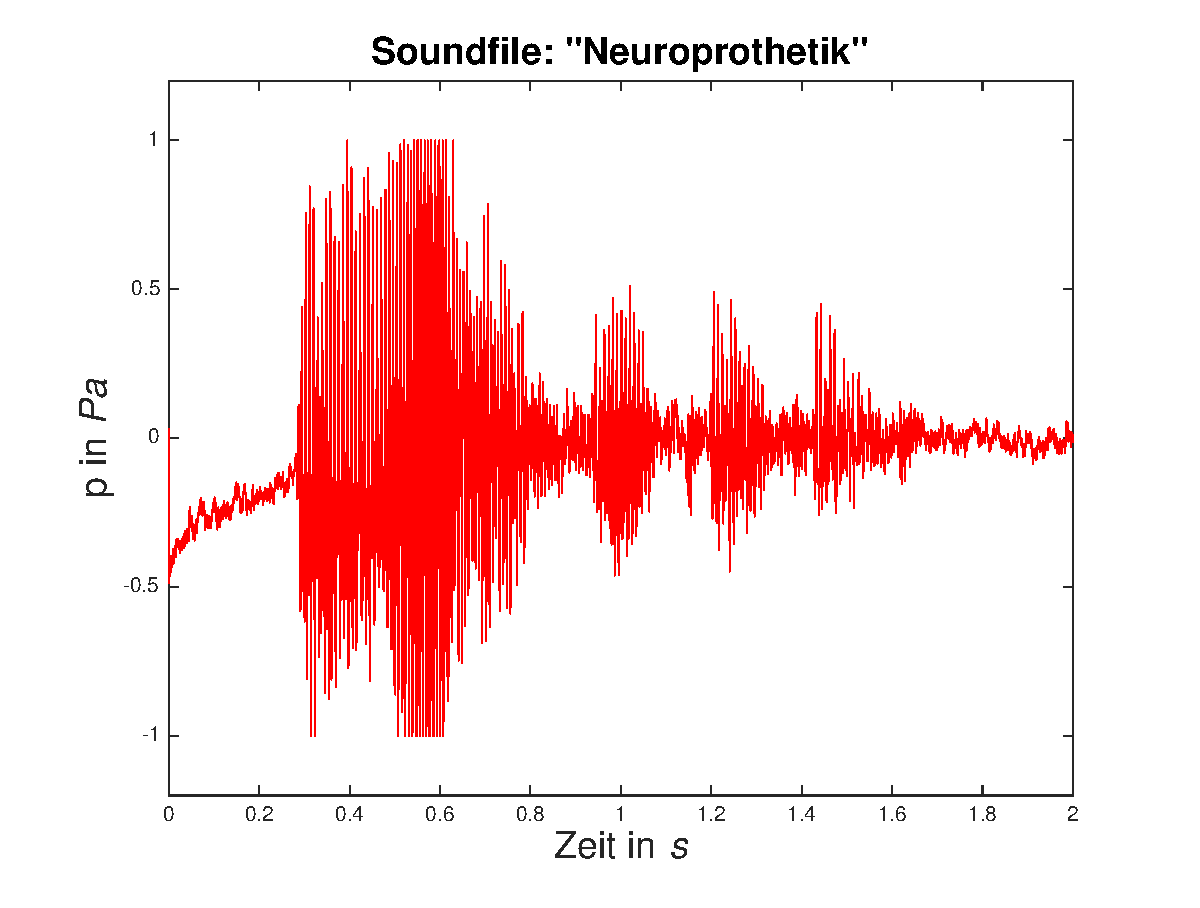
\includegraphics[width=0.7\linewidth]{Plots/orig_sound}
\caption{Darstellung des gesprochenen Wortes "Neuroprothetik" im Zeitbereich ohne Filterung.}
\label{fig:orig_sound}
\end{figure}

\subsection*{a)}
\begin{figure}[h]
\centering
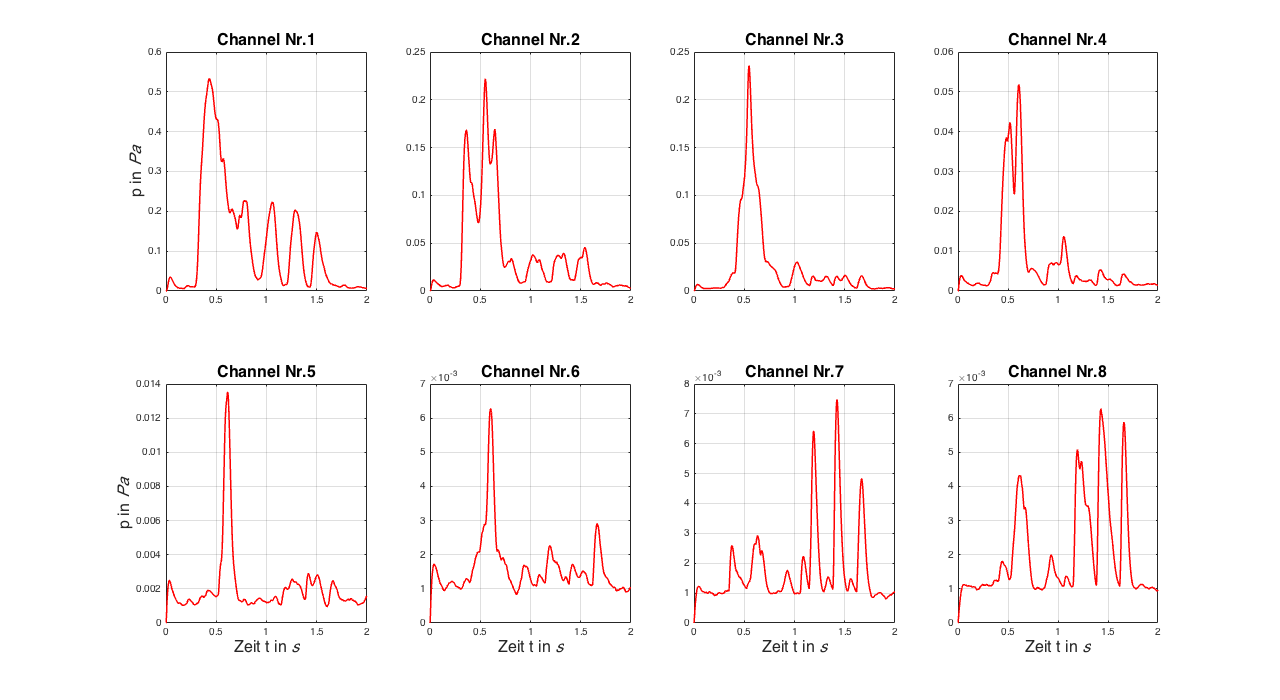
\includegraphics[width=1\linewidth]{Plots/a1_8ch}
\caption{Ausgang der 8-Kanal Einhüllendenextraktion mit Hilfe der Hilbert-Transformation und Tiefpassfilterung bei Eckfrequenz $f_{max}=30$ Hz.}
\label{fig:a1_8channels}
\end{figure}

\begin{figure}[h]
\centering
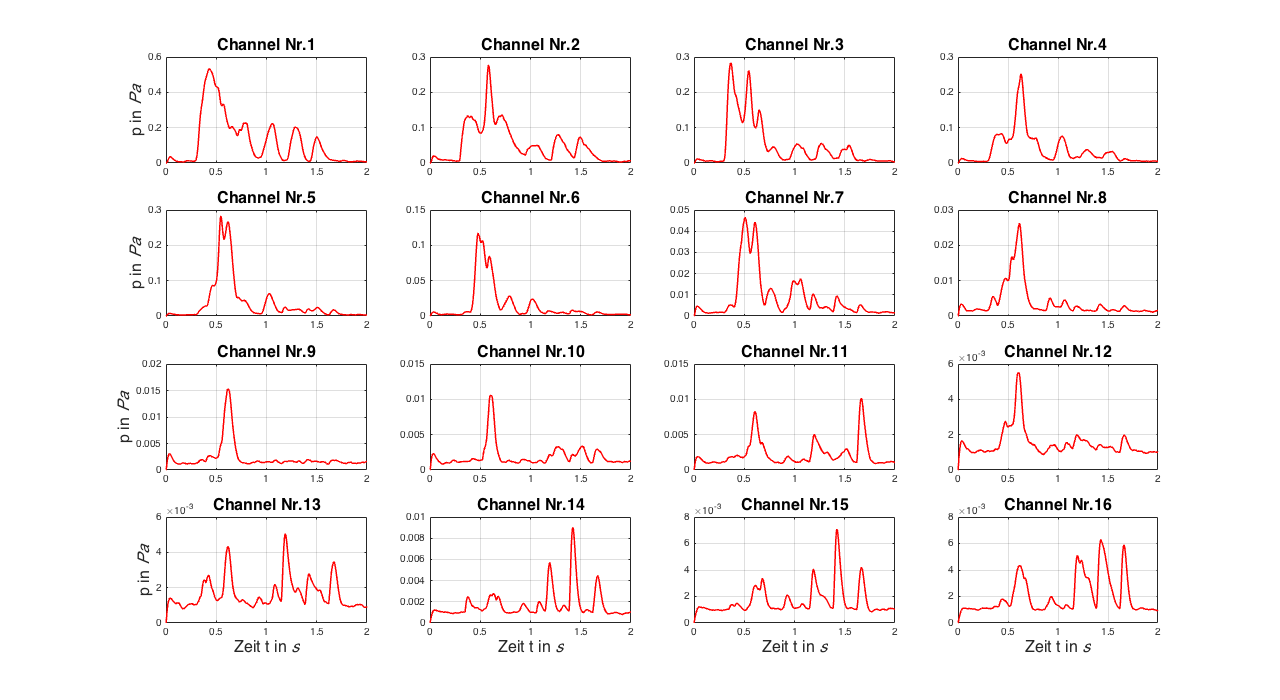
\includegraphics[width=1\linewidth]{Plots/a1_16ch}
\caption{Ausgang der 16-Kanal Einhüllendenextraktion mit Hilfe der Hilbert-Transformation und Tiefpassfilterung bei Eckfrequenz $f_{max}=30$ Hz.}
\label{fig:a1_16ch}
\end{figure}

\clearpage

\subsection*{b)}
\begin{figure}[h]
\centering
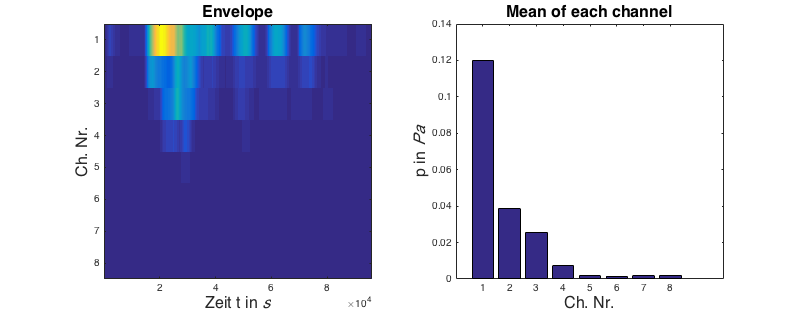
\includegraphics[width=0.9\linewidth]{Plots/b1_8ch}
\caption{8-Kanal-FB: Frequenzkanäle gegen die Zeit in Falschfarben (mit \texttt{imagesc()}-Befehl) und äquivalent zum Summenspektrum der mittlere Pegel über die Zeit für die einzelnen Kanäle.}
\label{fig:b1_8ch}
\end{figure}


\begin{figure}[h]
\centering
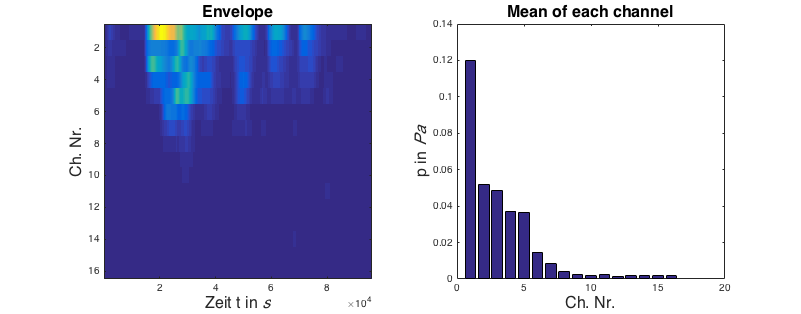
\includegraphics[width=0.9\linewidth]{Plots/b1_16ch}
\caption{16-Kanal-FB: Frequenzkanäle gegen die Zeit in Falschfarben (mit \texttt{imagesc()}-Befehl) und äquivalent zum Summenspektrum der mittlere Pegel über die Zeit für die einzelnen Kanäle.}
\label{fig:b1_16ch}
\end{figure}

\section*{Aufgabe 2}
\subsection*{a)}
\begin{figure}[h]
\centering
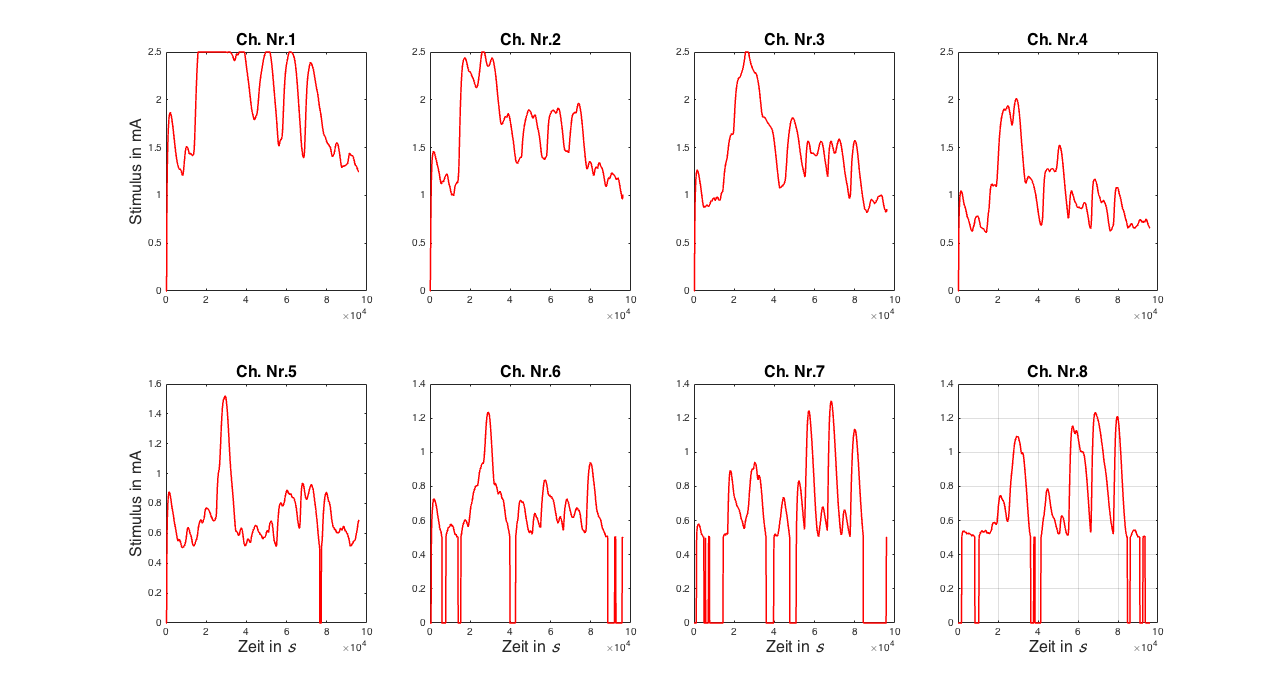
\includegraphics[width=1\linewidth]{Plots/a2_8ch}
\caption{8-Kanal-CI: Ausgang nach Dynamikkompression.}
\label{fig:a2_8ch}
\end{figure}

\begin{figure}[h]
\centering
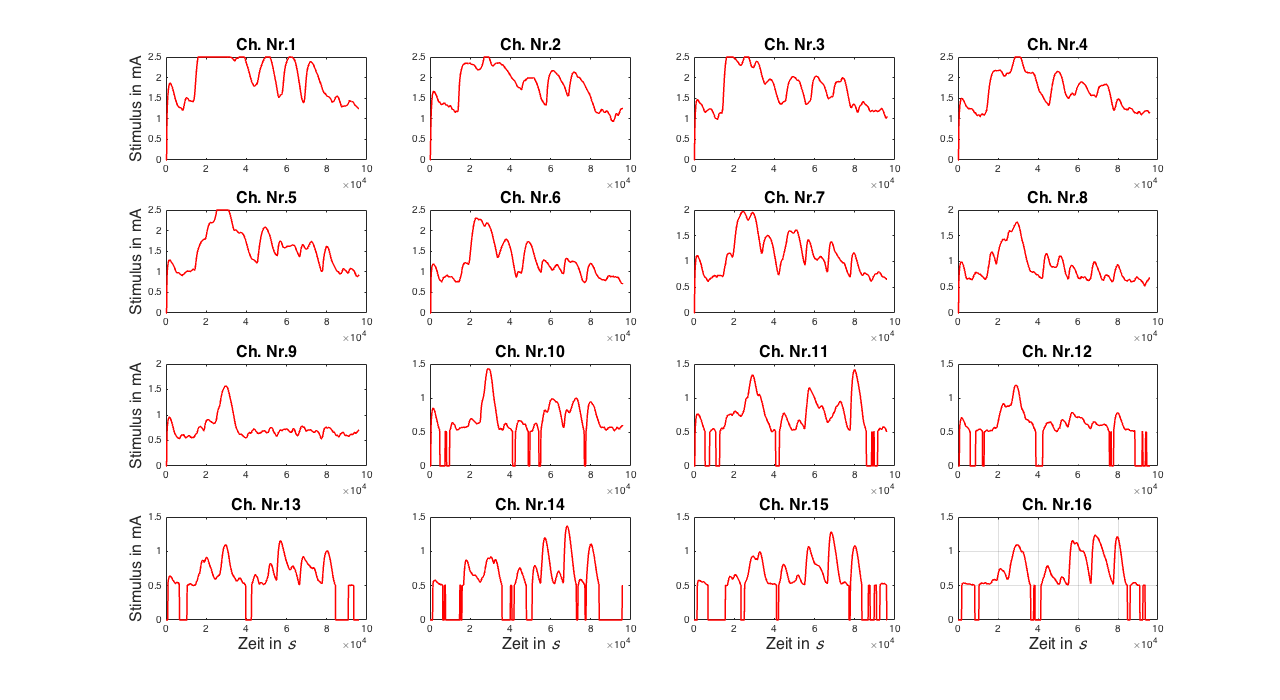
\includegraphics[width=1\linewidth]{Plots/a2_16ch}
\caption{16-Kanal-CI: Ausgang nach Dynamikkompression.}
\label{fig:a2_16ch}
\end{figure}

\clearpage
\subsection*{b)}
\begin{figure}[h]
\centering
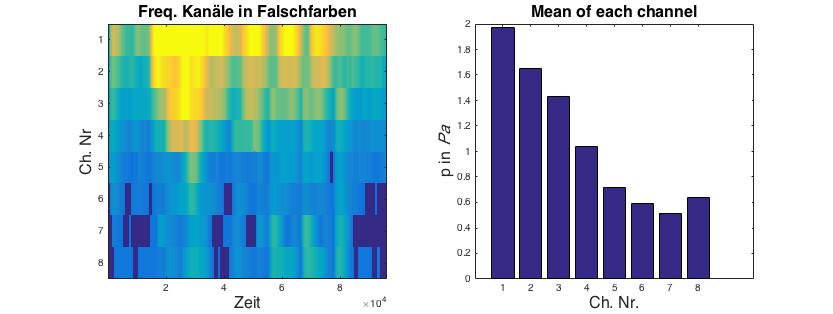
\includegraphics[width=0.9\linewidth]{Plots/b2_8ch}
\caption{Dynamische Kompression: 8-Kanal-FB: Frequenzkanäle gegen die Zeit in Falschfarben (mit \texttt{imagesc()}-Befehl) und äquivalent zum Summenspektrum der mittlere Pegel über die Zeit für die einzelnen Kanäle.}
\label{fig:b2_8ch}
\end{figure}

\begin{figure}[h]
\centering
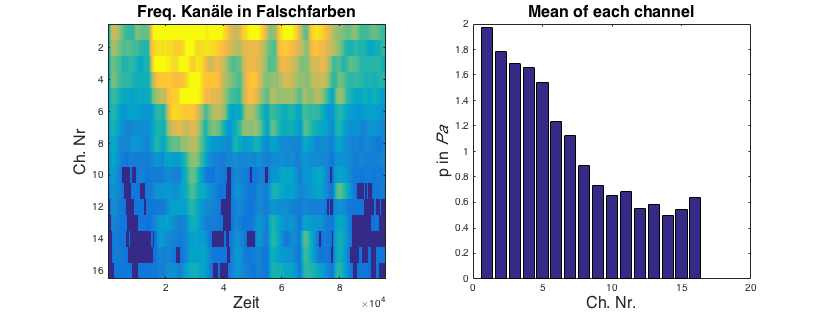
\includegraphics[width=0.9\linewidth]{Plots/b2_16ch}
\caption{Dynamische Kompression: 16-Kanal-FB: Frequenzkanäle gegen die Zeit in Falschfarben (mit \texttt{imagesc()}-Befehl) und äquivalent zum Summenspektrum der mittlere Pegel über die Zeit für die einzelnen Kanäle.}
\label{fig:b2_16ch}
\end{figure}

\clearpage
\subsection*{c)}
\begin{figure}[h]
\centering
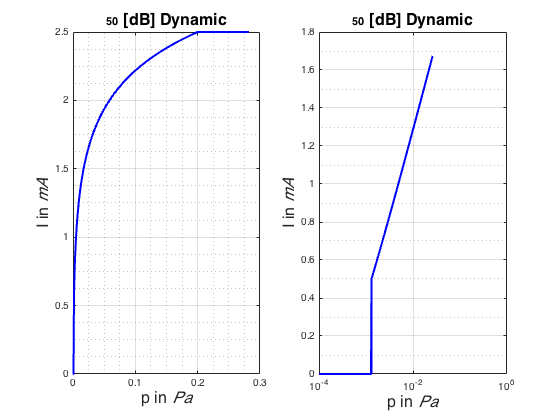
\includegraphics[width=0.6\linewidth]{Plots/c2_250}
\caption{Kompressionslinie der Dynamikkompression für $c = 250$}
\label{fig:c2_250}
\end{figure}

\begin{figure}[h]
\centering
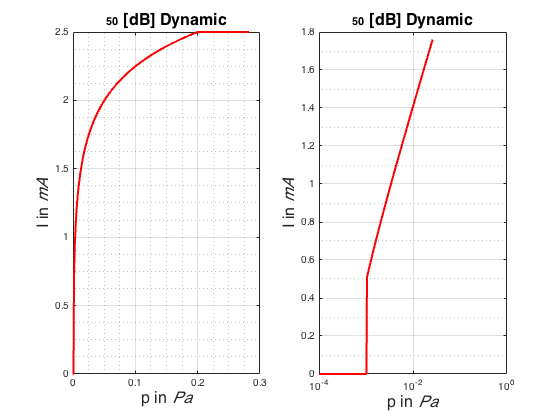
\includegraphics[width=0.6\linewidth]{Plots/c2_500}
\caption{Kompressionslinie der Dynamikkompression für $c = 500$}
\label{fig:c2_500}
\end{figure}

\begin{figure}[h]
\centering
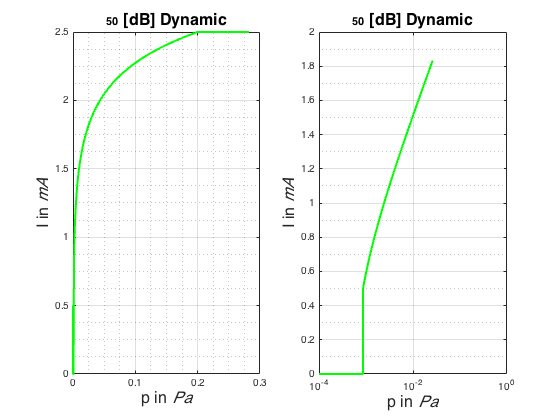
\includegraphics[width=0.6\linewidth]{Plots/c2_1000}
\caption{Kompressionslinie der Dynamikkompression für $c = 1000$}
\label{fig:c2_1000}
\end{figure}



\end{document}